\section{Foundations}

Our contributions are based on a preexisting approach to multi-model data modeling~\citep{mm_cat}. In this section, we introduce its main concepts and describe how it evolved into a comprehensive multi-model data management framework called \term{MM-cat}. But first, we need to explain some of the basic theory and terminology that we will be using throughout the thesis.

\subsubsection{Common terminology}

Let us define the levels of abstraction: \term{conceptual schema}, \term{logical models}, and \term{physical data}. The first is a \emph{platform-independent} representation of the business concepts. It doesn't limit the concepts to any specific data model or database system. The second is a \emph{platform-specific} representation of the data, tailored to a specific data model and database system---for example, a relational logical model cannot have nested structures, while a document logical model can. The last is the actual data stored in the database systems. We usually do not know its precise structure, as it is often an implementation detail of the specific database application.

Each data model (or even each database system) has its own terminology for the concepts and data structures it uses. Let us defined the following terms on the conceptual level:
\begin{itemize}
    \item \term{property} -- a basic concept with no internal structure (e.g., name, email),
    \item \term{entity} -- a structure consisting of properties (e.g., person, order),
    \item \term{relationship} -- a connection between an entity and a property or another entity (e.g., a person has a name, an order is for a person).
\end{itemize}
On the logical level, we use:
\begin{itemize}
    \item \term{kind} -- a class of items (e.g., a relational table, a collection of documents, or a node/edge label),
    \item \term{attribute} -- a property of a kind (e.g., a column in a table, a field in a document, or a property of a node/edge).
\end{itemize}
While kind has to correspond to an entity, an attribute can correspond to either an entity (e.g., a nested document in a document database) or a property (e.g., a column in a relational table). Relationships can be expressed in many different ways (e.g., references, nesting, inlining, etc.), so we do not define a unified term for them. Finally, on the physical level, we have:
\begin{itemize}
    \item \term{record} -- an item of a kind (e.g., a table row, a document, or a node/edge),
    \item \term{value} -- a value of an attribute in a record (e.g., a cell in a table row, a field in a document, or a property of a node/edge).
\end{itemize}

\subsubsection{Category Theory}

Category theory is a very abstract branch of mathematics that studies the properties of mathematical structures and their relationships. It provides a powerful framework for modeling and reasoning about complex systems, including data management systems.

The most important concept in the theory is the \term{category}. The full definition is in \Cref{cikm_2022:sec:conceptual-model}, but for the purpose of this introduction, we can think of a category as a directed multigraph---there is a set of nodes (called \term{objects}) and a set of directed edges (called \term{morphisms}) between them. Morphisms consisting of a single edge (we call them \term{base morphisms}) can be composed to more complex ones (\term{composite morphisms}).

A category can be mapped to another category via a \term{functor}, which is a mapping that preserves the structure of the categories. Formally, a functor is a function that maps each object in the first category to an object in the second category, and each morphism in the first category to a morphism in the second category, such that the composition of morphisms is preserved. The categories do not have to be the same size---for example, we can map multiple objects to a single object (and the morphisms between them to the identity morphism on that object). Or, we can map two objects connected by a base morphism to two objects connected by a composite morphism, which effectively expands the two objects into a more complex structure. In any case, the functor preserves the composition of morphisms, which is crucial for ensuring that objects in both categories have the same \emph{semantics}.

The previous paragraphs are obviously a gross oversimplification of the actual theory and its application in our research. There are many nuances and technical details that we do not cover here. Yet, if we want an approach to be actually useful, it is necessary to be able to explain it in a simple and intuitive way.

\subsection{MM-cat Framework}
\label{sec:mm-cat}

The basic idea of our approach is to create a \emph{unified model} of multi-model data on both conceptual and logical levels, and to use it as the basis for all the operations on the data, including querying and evolution. This unified model is based on category theory, which allows us to capture the semantics of all existing data models in a consistent way. The \term{MM-cat} framework is an implementation of this approach.

The conceptual schema is a category called \term{schema category}. Its objects represent the concepts in the domain of interest---entities and their properties, while its morphisms represent relationships between these concepts. An example of such category is shown in \Cref{fig:schema_category}. Each object has an internal identifier (not shown in the figure) and a label. By convention, entities have their labels capitalized (e.g., \object{User}) while properties have not (e.g., \object{id}). Morphisms can also have labels, but they are not displayed in the figure for simplicity. Instead, we distinguish them with \term{signatures} (in this case, integers). A signature like \signature{3.4} represents a composite morphism, which is a composition of the base morphisms with signatures \signature{3} and \signature{4}.

The previous version of schema category~\citep{mm_cat_journal} required that each morphism had a counterpart in the opposite direction (called \term{dual morphism}) and allowed each morhism to specify a \term{cardinality} in the same way as an \acrshort{er} would (e.g., \code{0..*}). The current version does have the concept of dual morphisms. Also, the cardinalities are limited to \code{0..1} and \code{1..1} in the direction of the morphism. For example, in \Cref{fig:schema_category}, we can immediatelly see that each instance of \object{User} can have at most one instance of \object{name} (even without providing any further information). This limitation is crucial to ensure that the conceptual schema can be mapped to any data model, because it requires each N:N relationship to be decomposed to an intermediate entity with two N:1 relationships. A more fine-grained cardinality control is achieved via categorical concepts like \term{monomorphism} and \term{epimorphism}.\\

\begin{figure}[ht]
    \centering
    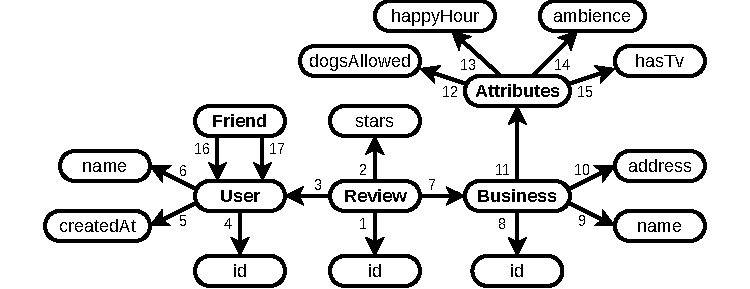
\includegraphics[width=\textwidth]{img/commentary-schema_category.drawio.pdf}
    \caption{An example of a schema category on the conceptual level, modelling a subset of the data from \Cref{fig:mm_data}. Objects (ovals) represent entities and properties, while morphisms (arrows) represent relationships between them. Each morphism has an integer signature. Identity morphisms (required by the definition of a category) are not shown for simplicity.}
    \label{fig:schema_category}
\end{figure}

On the logical level, each kind has its own logical model. A logical model is also a schema category, but it is defined over a specific data model and database system. Therefore, its objects and morphisms have a very specific semantics, e.g., in a relational model, there would be an entity representing the table, properties representing its columns, and morphisms between them meaning that the columns belong to the table. Because the underlying kinds are always trees, the schema categories of logical models are also trees with a distinguished \term{root object}. An example of a logical model for a columnar database is shown in \Cref{fig:mapping}.

The schema category has to conform to the constraints of the underlying data model. For example, in a relational model, columns cannot contain array values, so there cannot be a morphism from a column object to the table object. However, in a document model, there is no such restriction, so we can have a morphism from a field object to a document object, representing the fact that the field is an array nested inside the document.\\

\begin{figure}[ht]
    \centering
    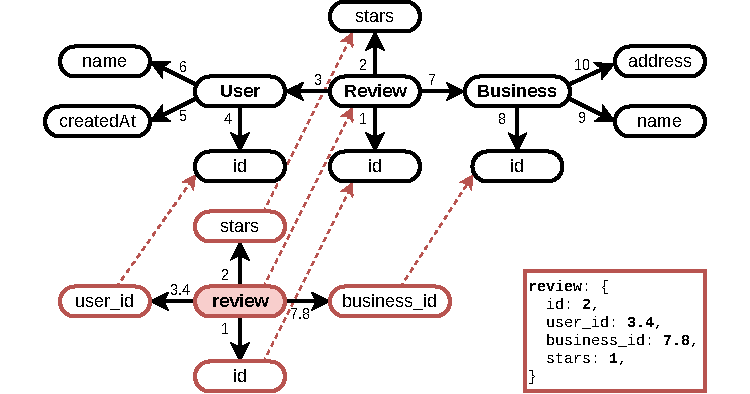
\includegraphics[width=\textwidth]{img/commentary-mapping.drawio.pdf}
    \caption{An example of a logical model for a columnar database (red), mapped to the conceptual schema from \Cref{fig:schema_category} via a functor. Because the schema category of the logical model is a tree, we can express both it and its mapping to the conceptual schema in a single \acrshort{json}-like document (on right).}
    \label{fig:mapping}
\end{figure}

Finally, each logical model is connected to the conceptual schema via a \term{mapping}, which is a functor that maps objects and morphisms between both schema categories (from the logical model to the conceptual schema) while preserving their structure. For example, the \Cref{fig:mapping} shows a mapping from the logical model of a columnar database to the conceptual schema from \Cref{fig:schema_category}. A logical model for a table \object{review} cannot have a column \object{user}, because user is an entity and columnar model does not support nested structures. However, we can \term{inline} the \object{id} property into the \object{review} table by using a logical model with objects \object{review} and \object{user\_id} (mapped to \object{Review} and \object{id} from the conceptual schema), and a morphism between them (mapped to the composite morphism from \object{Review} to \object{id} in the conceptual schema).

Besides the structural changes, the mapping can also rename objects---for example, to conform to the naming conventions of the underlying database system, or to avoid name clashes with attributes of different kinds.

\subsubsection{Tools}

MM-cat framework is an umbrella term for a family of tools based on the above-described unified representation. The first one, also called \term{MM-cat}~\citep{mm_cat}, enables multi-model data modeling, as well as transformation of data between various models. The second one, \term{MM-evocat} (\paperRef{cikm_2022}), adds the ability to evolve the conceptual schema and propagate changes. \term{MM-infer}~\citep{mm_infer}, later extended in \paperRef{enase_2025, edbt_2025}, allows to infer the conceptual schema and logical models from the data. \term{MM-quecat}~\citep{mm_quecat} resp. \term{MM-evoque} (\paperRef{edbt_2024}) enables querying multi-model data using a unified query language resp. propagating changes from the conceptual schema to the queries. Finally, \term{MM-mapsearch} (\paperRef{edbt_2026}) explores the concept of self-adaptation.

The overall architecture of the system is shown in \Cref{fig:architecture}. The tools roughly correspond to the milestones from \Cref{sec:vision}, however, in practice they are more of different \emph{use cases} of one unified system than a set of separated tools. This proof-of-concept implementation is crucial for testing the proposed approach and demonstrating its feasibility.

\begin{figure}[ht]
    \centering
    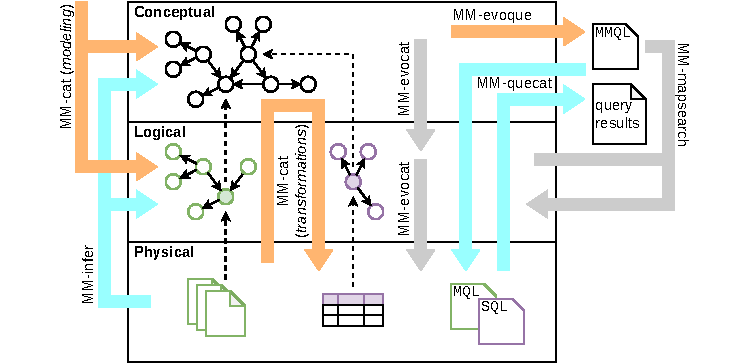
\includegraphics[width=\textwidth]{img/commentary-architecture.drawio.pdf}
    \caption{Architecture of the MM-cat framework, showing the main tools and their interactions. The arrows represent the flow of data and control between the artifacts on the three levels of abstraction. The colors of the arrows don't have any particular meaning.}
    \label{fig:architecture}
\end{figure}

\subsection{Querying}
\label{sec:querying}

Each database system has its own query language, tailored to the specific data model. From SQL to XQuery, these languages have vast differences in both syntax and semantics. Even within the same data model, query languages (e.g., SPARQL and Cypher for the graph model) offer very diverse features.

Mastering multiple query languages takes a lot of time and effort, and it is not realistic to expect users to be proficient in all of them. This is a huge barrier for using multi-model data efficiently. Therefore, we want to be able to query multi-model data using a single, unified query language. Such a language should be expressive enough to cover all queries across all data models, and it should recognize all possible data structures that can be returned by these queries.

Lastly, one of the primary motivations for using multi-model data is the performance benefits from using the best model for the given job. In order to fully realize these benefits, the overhead of using the unified query language should be minimal, ideally negligible compared to a native solution.

\subsubsection{MMQL}

These requirements led us to the development of \term{MMQL} (\textbf{M}ulti-\textbf{m}odel \textbf{q}uery \textbf{l}anguage)~\citep{mm_quecat, koupil2023universal}. MMQL is a query language over the schema category, making it independent both of the underlying data models and of the specific databases. After parsing, the query engine splits the query into maximal subqueries that can be executed on a single database, translates them to the native query languages, executes them, and finally combines the results together.

The syntax of MMQL is based on SPARQL, as it is a well-known and widely used query language for graph data (and schema category can be represented as a multigraph). Each triple pattern in the query corresponds to a morphism in the schema category, together with its domain and codomain objects. However, the similarity to SPARQL is just syntactic, as both objects and morphisms in the schema category can have very different semantics dependent on the underlying data models and databases. E.g., one morphism can represent a join in a relational database, a relationship kind in a property graph database, or a nested document in a document database. An example of MMQL query is displayed in \Cref{fig:querying}.

\begin{figure}[ht]
    \centering
    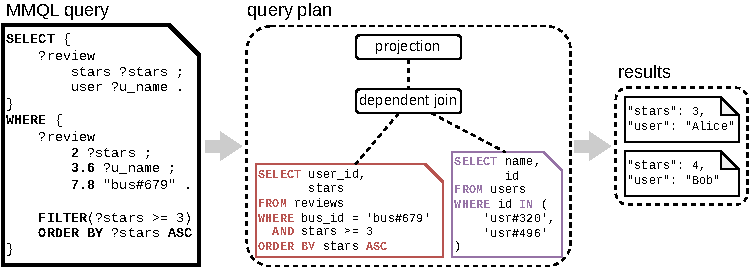
\includegraphics[width=\textwidth]{img/commentary-querying.drawio.pdf}
    \caption{Example of MMQL over the schema category from \Cref{fig:schema_category}. In the \code{WHERE} clause, we express the pattern to match via the signatures of the morphisms. We can also filter, order, or group the data. The \code{SELECT} describes the structure of the result.}
    \label{fig:querying}
\end{figure}

A single \term{query plan} is created by matching the patterns in the query to the available logical models (via the mappings from the schema category). In case of multiple possible combinations (i.e., if the same data is stored in multiple databases), multiple query plans are created and the best one is chosen based on the estimated cost.

Optimizations play a crucial role in this process. We have explored, implemented, and evaluated several techniques to improve the performance of MMQL queries~\citep{strobl-mastersthesis}:

\begin{itemize}
    \item \term{Predicate pushdown} -- Generally, it is more efficient to filter the data as early as possible, ideally in the underlying databases, so we push the predicates down along the query plan tree. Not all operations can be pushed to the databases (e.g., cross-database joins), so they are executed in the query engine. In some cases, the databases do not support certain operations (e.g., aggregation), or they might not be very efficient (e.g., lookups in MongoDB), so we have to execute them by ourselves as well.
    \item \term{Dependent joins} -- If one side of a join depends on the results of the other side, we might be able to push this as a \uv{filter} to the database. E.g., when two kinds are joined on a key, we can query one of them first and then use the possible key values as a filter for the second one. This is especially beneficial when the first kind is already heavily filtered by other predicates.
    \item \term{Cost estimation} -- The cost of plans and subplans is the most important factor for plan creation and selection. We have implemented cache-based cost estimation, allowing us to reuse the results of previous queries and to learn from them over time. We have also implemented a simple cost model based on the cost estimated by the databases and the number of records processed by each operation, which is used when there is no information in the cache.
\end{itemize}

\subsection{Related Work}
\label{sec:foundations-related-work}

\todo{RELATED WORK - this part is work in progress}

Traditionally, relational data is modeled using \acrshort{er} or \acrshort{uml} diagrams. Even though they are not expressive enough to capture all the semantics of multi-model data\footnotei{For example, key-value maps representing a number of dynamic attributes of an entity/class.}{,} they are still widely used in practice so we can at least use them as an inspiration. Other aspects of data management (evolution, querying, etc.) are usually specific to a particular database system, and therefore they are not directly applicable to multi-model data.\\

\term{U-schema}~\citep{DBLP:journals/is/CandelRM22} offers a unified representation for multi-model data. It is a foundation for the \term{Orion} language~\citep{DBLP:conf/er/ChillonRM21a, 10.1109/TKDE.2024.3362273}, enabling evolution, and \term{SkiQL}~\citep{skiql}, enabling querying the schema. Although these capabilities might sound very similar to the ones we propose in this thesis, there are a few important differences.

First, U-schema tries to unify the data models on the \emph{logical} rather than the \emph{conceptual} level. This leads either to an inability to tailor the representation to the specific features of each data model (if we use one logical model for multiple databases), or to a redundancy and a loss of semantics (if we use multiple disconnected logical models). We try to avoid this issue by using a unified conceptual schema that is independent of the underlying data models, and then mapping it to the specialized logical models. Similarly, the evolution only happens on the logical level, so the evolution propagation to data is much more straightforward.

A biggest difference is in the querying capabilities. SkiQL is a \emph{schema} query language, which means that it can only query the structure of the data, but not its content. This is a very important distinction, as our focus is on the opposite---we only query the contents of the data, not its structure. However, this is not a limitation of our approach, as we can still get the structure either from our internal model or from the data (i.e., by inference).\\

There is also a more theoretical approach~\citep{DBLP:journals/corr/abs-2201-04905}. It describes multi-model data and their transfomations in the terms of category theory, but it does not provide any practical tools for managing multi-model data. A recently published version~\citep{lu2025part1, lu2025part2} is much more rigorous and comprehensive while also exploring querying multi-model data. It introduces categorical algebra and calculus as an extension of relational algebra and calculus via multi-model predicates.

\todo{
    Podívat se ještě na Gallinucci, podle Pavla se nám blíží nejvíc.

    E. Gallinucci, M. Golfarelli, S. Rizzi, A. Abelló, O. Romero, Interactive multidimensional modeling of linked data for exploratory OLAP, Inf. Syst. 77 (2018) 86–104. doi:10.1016/J.IS.2018.06.004.
}

\subsection{Contributions}

As mentioned above, this section serves as a summary of a previous research that we used as the basis for our work, so we do not claim many contributions here. What we do claim is the proof-of-concept implementation of the MM-cat framework, evaluation of the proposed approach, and a refinement of the original model.

Besides that, we have also contributed to the development of the MMQL query language by solidifying its syntax and semantics, implementing it in the query engine, and optimizing its performance using the techniques described in \Cref{sec:querying}.
